% Archivo temporal con el contenido de la imagen TEOREMA_NORTON-07.png

\section*{Teorema de Norton}
\pagenumbering{gobble} % Opcional: para quitar el número de página si se compila solo
\pagestyle{empty} % Opcional: para quitar cabeceras/pies de página

\begin{figure}[h!]
    \centering
    % 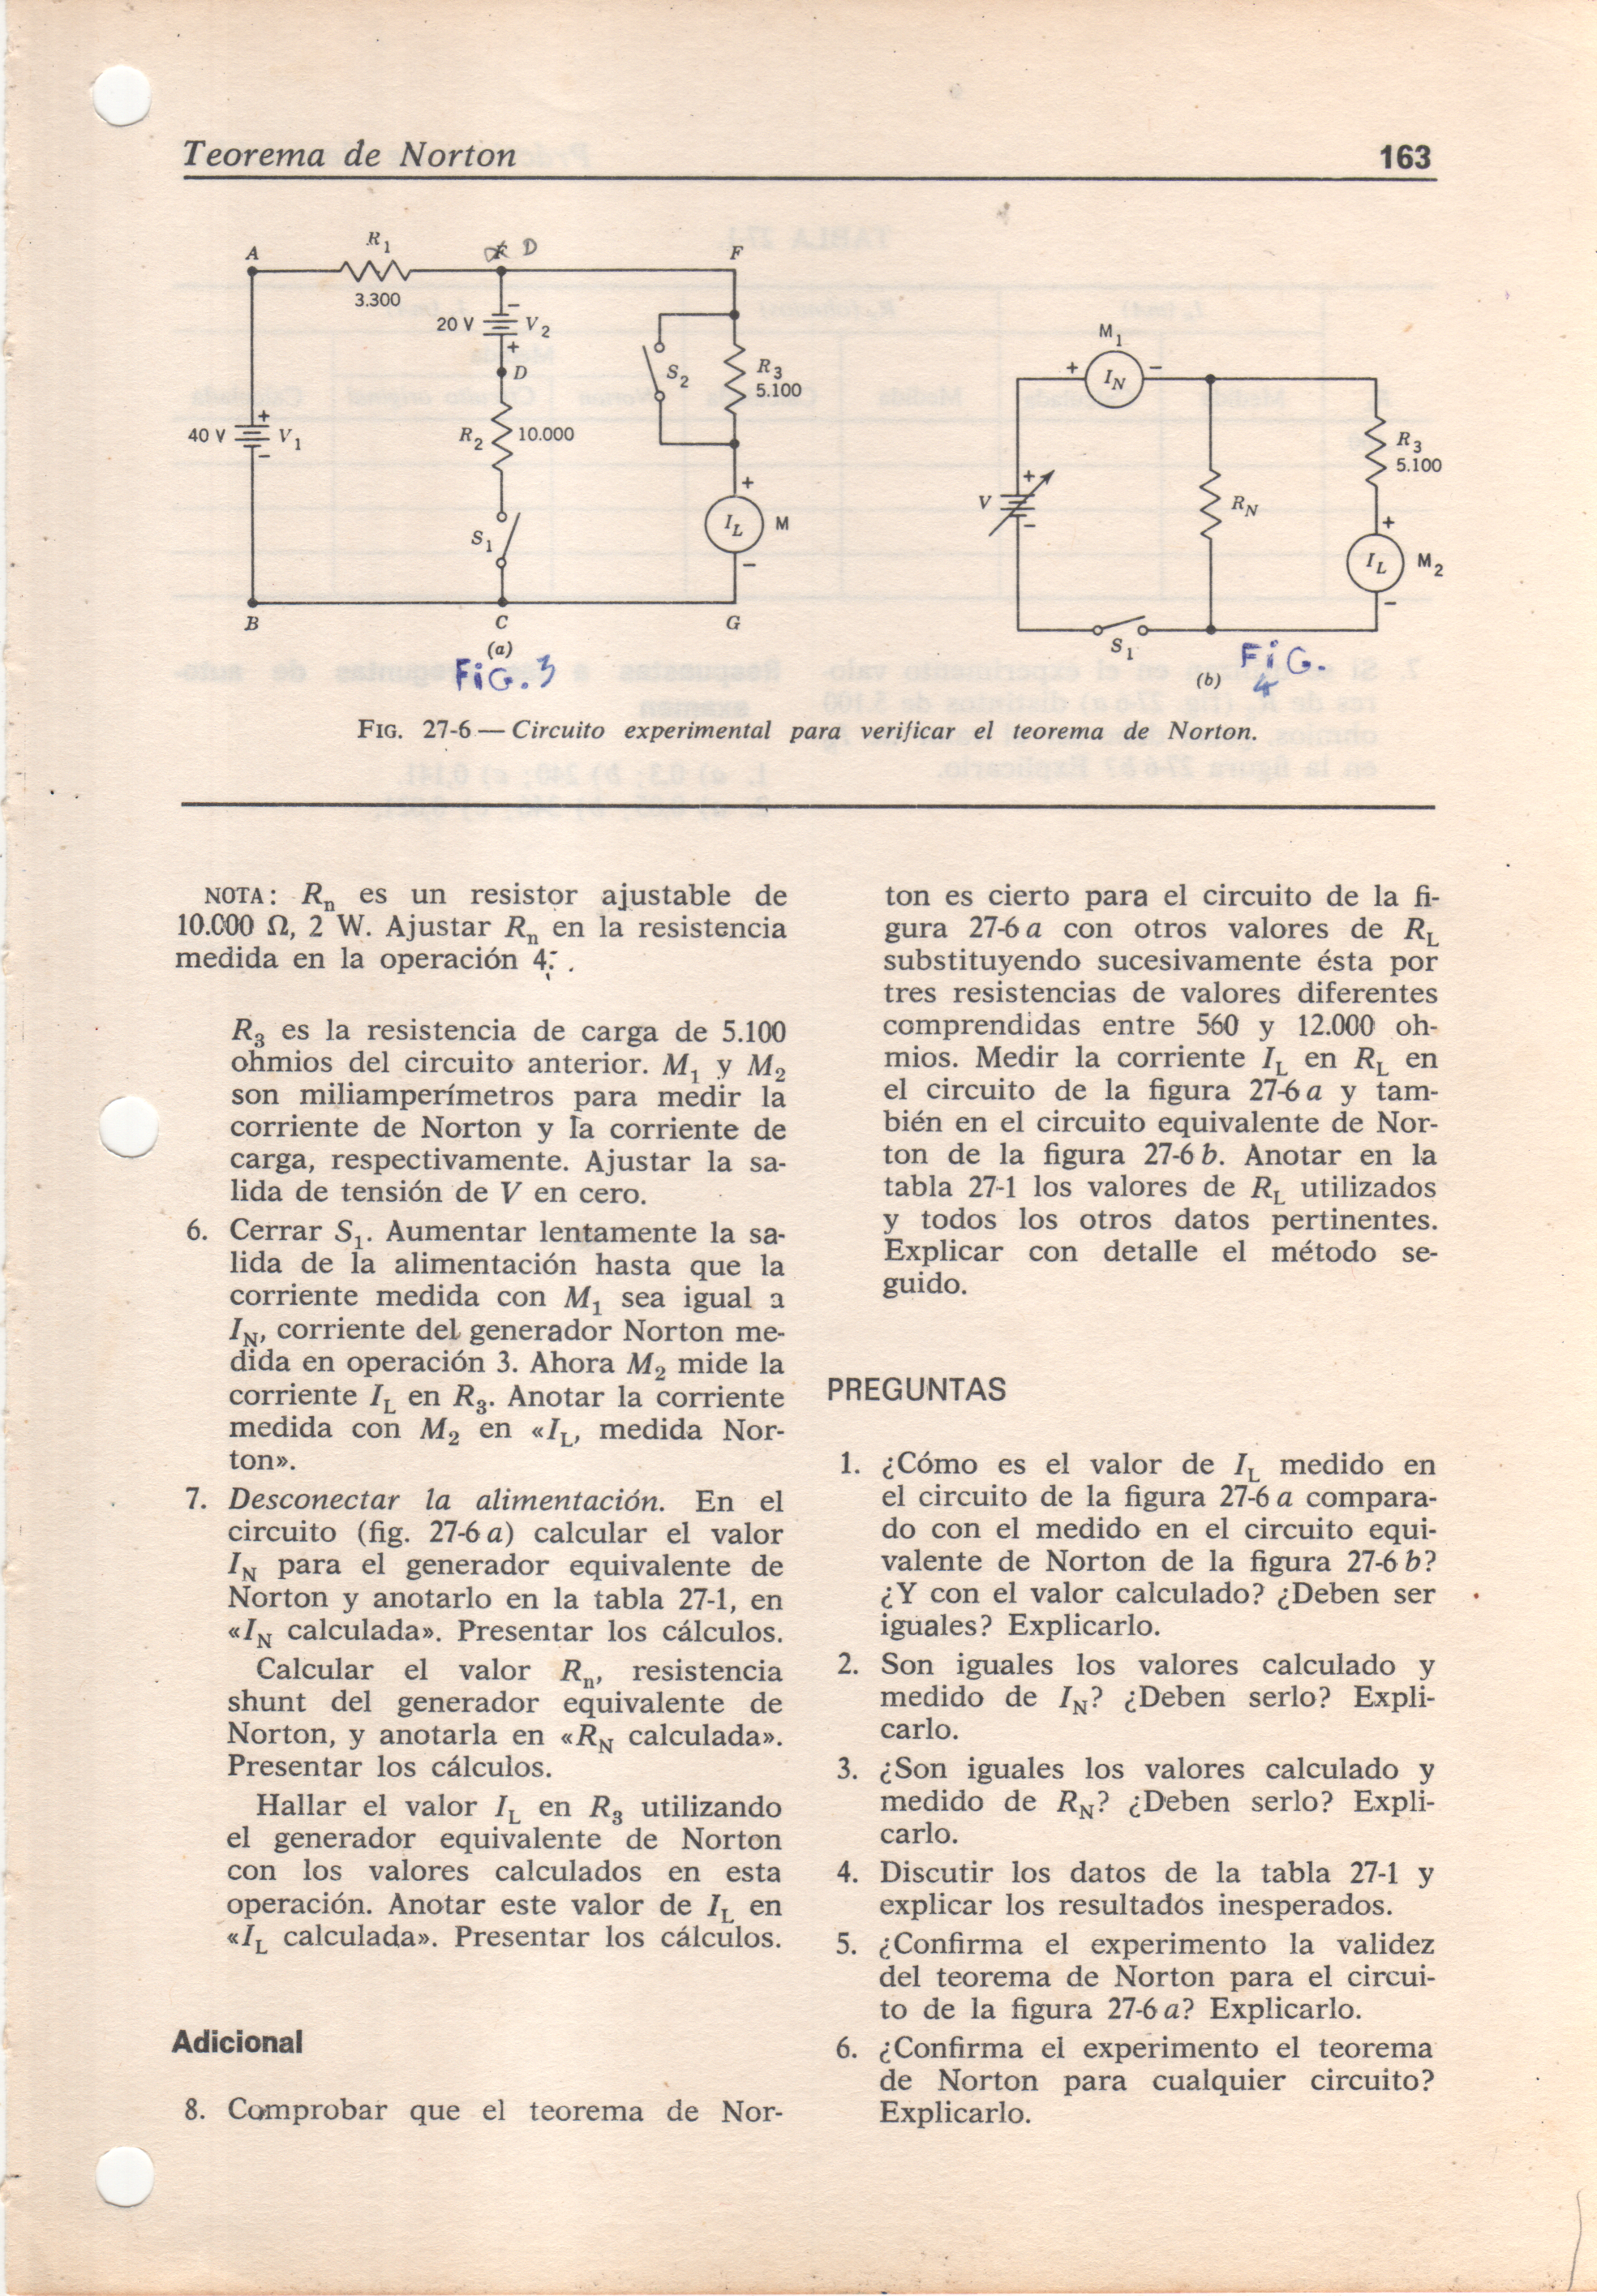
\includegraphics[width=\textwidth]{imagenes/TEOREMA_NORTON-07.png}
    \vspace{5cm} % Espacio vertical para las imágenes
    \textbf{[ESPACIO PARA IMAGEN: Circuitos (a) y (b)]}
    \caption{Circuito experimental para verificar el teorema de Norton.}
    \label{fig:circuito_experimental_norton}
\end{figure}

\noindent
\textbf{NOTA:} $R_N$ es un resistor ajustable de \SI{10000}{\ohm}, \SI{2}{\watt}. Ajustar $R_N$ en la resistencia medida en la operación 4.

\vspace{1em} % Un pequeño espacio vertical

\noindent
$R_3$ es la resistencia de carga de \SI{5100}{\ohm} del circuito anterior. $M_1$ y $M_2$ son miliamperímetros para medir la corriente de Norton y la corriente de carga, respectivamente. Ajustar la salida de tensión de V en cero.

\begin{enumerate}[resume, label=\arabic*.]
    \setcounter{enumi}{5} % Empezamos la lista en el número 6
    \item Cerrar $S_1$. Aumentar lentamente la salida de la alimentación hasta que la corriente medida con $M_1$ sea igual a $I_N$, corriente del generador Norton medida en operación 3. Ahora $M_2$ mide la corriente $I_L$ en $R_3$. Anotar la corriente medida con $M_2$ en «$I_L$, medida Norton».

    \item Desconectar la alimentación. En el circuito (fig. 27-6 a) calcular el valor $I_N$ para el generador equivalente de Norton y anotarlo en la tabla 27-1, en «$I_N$ calculada». Presentar los cálculos.

    Calcular el valor $R_N$, resistencia shunt del generador equivalente de Norton, y anotarla en «$R_N$ calculada». Presentar los cálculos.

    Hallar el valor $I_L$ en $R_3$ utilizando el generador equivalente de Norton con los valores calculados en esta operación. Anotar este valor de $I_L$ en «$I_L$ calculada». Presentar los cálculos.
\end{enumerate}

\subsection*{Adicional}
\begin{enumerate}[resume, label=\arabic*.]
    \item Comprobar que el teorema de Norton es cierto para el circuito de la figura 27-6 a con otros valores de $R_L$ substituyendo sucesivamente ésta por tres resistencias de valores diferentes comprendidas entre 560 y \SI{12000}{\ohm}. Medir la corriente $I_L$ en $R_L$ en el circuito de la figura 27-6 a y también en el circuito equivalente de Norton de la figura 27-6 b. Anotar en la tabla 27-1 los valores de $R_L$ utilizados y todos los otros datos pertinentes. Explicar con detalle el método seguido.
\end{enumerate}

\section*{PREGUNTAS}
\begin{enumerate}[label=\arabic*.]
    \item ¿Cómo es el valor de $I_L$ medido en el circuito de la figura 27-6 a comparado con el medido en el circuito equivalente de Norton de la figura 27-6 b? ¿Y con el valor calculado? ¿Deben ser iguales? Explicarlo.

    \item ¿Son iguales los valores calculado y medido de $I_N$? ¿Deben serlo? Explicarlo.

    \item ¿Son iguales los valores calculado y medido de $R_N$? ¿Deben serlo? Explicarlo.

    \item Discutir los datos de la tabla 27-1 y explicar los resultados inesperados.

    \item ¿Confirma el experimento la validez del teorema de Norton para el circuito de la figura 27-6 a? Explicarlo.

    \item ¿Confirma el experimento el teorema de Norton para cualquier circuito? Explicarlo.
\end{enumerate}